\documentclass[aps,prb,onecolumn,nofootinbib]{revtex4-2}

\usepackage{amsmath,amssymb,mathtools,bm}
\usepackage{graphicx}
\usepackage{hyperref}
\usepackage{xcolor}

\newcommand{\triv}{\mathrm{triv}}
\newcommand{\topo}{\mathrm{top}}
\newcommand{\dw}{\mathrm{DW}}
\newcommand{\ii}{\mathrm{i}}
\newcommand{\dd}{\mathrm{d}}
\newcommand{\Id}{\mathbf{1}}
\newcommand{\Ay}{A_y}
\newcommand{\LB}{l_B}
\newcommand{\LA}{L_A}
\newcommand{\LC}{L_C}
\newcommand{\Ix}{I_x}
\newcommand{\SA}{S_A}

\begin{document}

\title{Exact Domain-Wall Ground-State Benchmark for a Lattice Chern Insulator}
\author{Asad and GPT-5.4 Codex}
\date{\today}

\begin{abstract}
This note collects the formulas used in the notebook
\texttt{notebooks/exact\_DW\_GS\_benchmark.ipynb} and organizes them into a
single theoretical narrative.  The benchmark concerns an exactly solvable
Gaussian ground state of a real-space domain-wall Chern-insulator Hamiltonian,
its momentum-resolved and boundary-resolved spectra, the entanglement contour,
fixed-$x$ squared-correlation profiles, the local Chern marker,
strip-integrated contour diagnostics, and a
contour-restricted multipartite-information construction.  All figures presently
stored in \texttt{DW\_GS\_Benchmark\_Figs/} are included with captions.
\end{abstract}

\maketitle

\section{Model and Domain-Wall Geometry}
The notebook studies a two-orbital free-fermion model on an
$N_x \times N_y$ square lattice.  At each unit cell $(x,y)$ one introduces the
spinor
\begin{equation}
\Psi_{x,y}
=
\begin{pmatrix}
c_{x,y,0} \\
c_{x,y,1}
\end{pmatrix},
\end{equation}
and uses the site-orbital flattening convention
\begin{equation}
i(\mu,x,y) = \mu + 2x + 2N_x y,
\qquad
\mu \in \{0,1\}.
\end{equation}

The notebook convention is
\begin{equation}
\alpha_{\triv} \equiv \alpha_1,
\qquad
\alpha_{\topo} \equiv \alpha_2,
\end{equation}
with the domain-wall slab generated by the code path
\texttt{create\_domain\_wall}.  In the default construction the mass profile is
\begin{equation}
\alpha(x,y) =
\begin{cases}
\alpha_{\topo}, & x_0 \le x \le x_1,\\
\alpha_{\triv}, & \text{otherwise},
\end{cases}
\label{eq:alpha-profile}
\end{equation}
where the two domain-wall positions are stored as
\begin{equation}
\mathrm{DW\_loc} = [x_0, x_1].
\end{equation}
In the code this slab is centered near $x=N_x/2$ and its width is chosen as an
$\mathcal{O}(0.2N_x)$ fraction of the system size.

The real-space Hamiltonian used by the exact benchmark is
\begin{align}
H
&=
\sum_{x,y}
\Psi_{x,y}^{\dagger}
\bigl[\alpha(x,y)\sigma_z \bigr]
\Psi_{x,y}
\nonumber\\
&\quad
+ \sum_{x,y}
\Bigl(
\Psi_{x,y}^{\dagger}\, t_x \,\Psi_{x+1,y}
+
\Psi_{x,y}^{\dagger}\, t_y \,\Psi_{x,y+1}
+
\mathrm{h.c.}
\Bigr),
\label{eq:realspace-h}
\end{align}
with nearest-neighbor matrices
\begin{equation}
t_x = -\frac{1}{2}\sigma_z - \frac{\ii}{2}\sigma_x,
\qquad
t_y = -\frac{1}{2}\sigma_z - \frac{\ii}{2}\sigma_y.
\label{eq:hopping-blocks}
\end{equation}
For a spatially uniform mass $\alpha$ this corresponds to the familiar Bloch
Dirac-Chern form
\begin{equation}
h(\bm{k})
=
\sin k_x\, \sigma_x
+
\sin k_y\, \sigma_y
+
\bigl(\alpha - \cos k_x - \cos k_y \bigr)\sigma_z.
\label{eq:bloch-h}
\end{equation}

\section{Continuum Edge Expectation: Chiral Free Fermion in \texorpdfstring{$1+1$}{1+1}D}
The domain-wall benchmark is motivated by the expectation that each interface
supports a low-energy chiral boundary mode.  In continuum language, the
universal fixed point is a chiral free fermion conformal field theory in
$1+1$ dimensions.  The chiral fermion field $\psi$ has scaling dimension
\begin{equation}
h = \frac{1}{2},
\end{equation}
so on a spatial circle of circumference $L$ its equal-time two-point function
has the standard chord-length form
\begin{equation}
\langle \psi^\dagger(y)\psi(0)\rangle
\propto
\frac{1}{\sin(\pi y/L)},
\label{eq:chiral-fermion-two-point}
\end{equation}
up to a phase and a nonuniversal amplitude.  Consequently, the squared
magnitude obeys
\begin{equation}
\bigl|\langle \psi^\dagger(y)\psi(0)\rangle\bigr|^2
\propto
\sin^{-2}(\pi y/L).
\label{eq:chiral-fermion-squared}
\end{equation}
This is the continuum reason that a lattice observable dominated by a single
chiral edge mode is expected to yield slope $-2$ when plotted as
$\log C$ versus the logarithm of a periodic chord length.  The squared
correlation diagnostics below test precisely how well that expectation is
realized, and over what spatial range in $x$ it remains valid near the two
domain walls.

The notebook also exposes an optional flag
\texttt{triv\_region\_local\_mode}.  In that branch the complement of the
domain-wall slab is replaced by decoupled onsite modes, with onsite block
$-\Id_2$, and all hoppings touching that region are removed.  Since the figures
stored in the benchmark directory were generated from the standard branch, the
main text below focuses on Eqs.~\eqref{eq:alpha-profile}--\eqref{eq:hopping-blocks}.

\section{Exact Gaussian Ground State}
The equilibrium covariance is obtained by diagonalizing the single-particle
Hamiltonian,
\begin{equation}
H u_n = E_n u_n,
\end{equation}
forming the occupied-state projector
\begin{equation}
P_- = \sum_{E_n < 0} |u_n\rangle \langle u_n|,
\label{eq:pminus}
\end{equation}
and finally constructing the flattened covariance matrix
\begin{equation}
G = 2P_- - \Id.
\label{eq:covariance}
\end{equation}
This is precisely the object returned by
\texttt{G\_CI\_domain\_wall}.  At half filling, Eq.~\eqref{eq:covariance}
encodes the entire Gaussian state.

The notebook supplements the raw ordered spectrum of $H$ by a momentum-resolved
diagnostic along $y$.  One reshapes the flattened matrix into
\begin{equation}
G(x,y,\mu; x',y',\nu),
\end{equation}
performs a unitary Fourier transform on the bra $y$ index and an inverse
transform on the ket $y'$ index,
\begin{equation}
\widetilde{G}(x,k_y,\mu;x',k_y',\nu)
=
\frac{1}{N_y}
\sum_{y,y'}
e^{-\ii k_y y}\,
G(x,y,\mu;x',y',\nu)\,
e^{+\ii k_y' y'},
\label{eq:ky-transform}
\end{equation}
and then extracts the contiguous $(2N_x)\times(2N_x)$ blocks associated with
fixed $k_y$ in the notebook's flattening convention.  The same procedure is
applied to $H$ for the displayed energy bands versus $k_y/\pi$.

\begin{figure}[t]
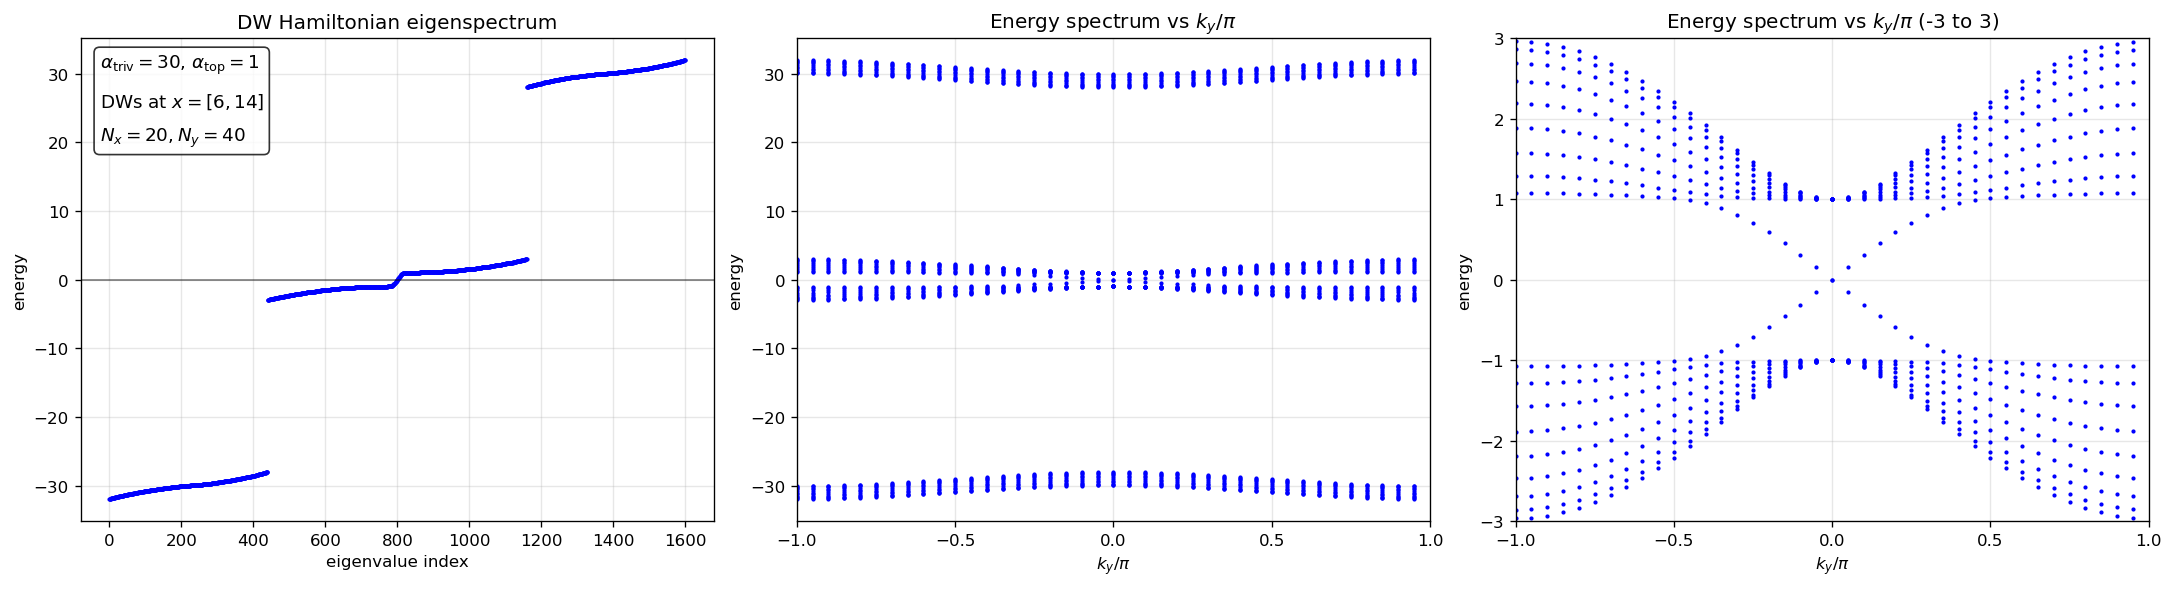
\includegraphics[width=\textwidth]{DW_GS_Benchmark_Figs/energy_spec.fig.png}
\caption{
Exact periodic-boundary spectrum for the benchmark geometry
$N_x=20$, $N_y=40$, with $\alpha_{\triv}=30$, $\alpha_{\topo}=1$, and
domain walls at $x\in[6,14]$.
Left: ordered eigenvalues of the real-space Hamiltonian.
Middle: spectrum of the $k_y$-resolved blocks obtained from the transform
\eqref{eq:ky-transform}.
Right: the same spectrum restricted to a low-energy window.
}
\label{fig:energy-main}
\end{figure}

\begin{figure}[t]
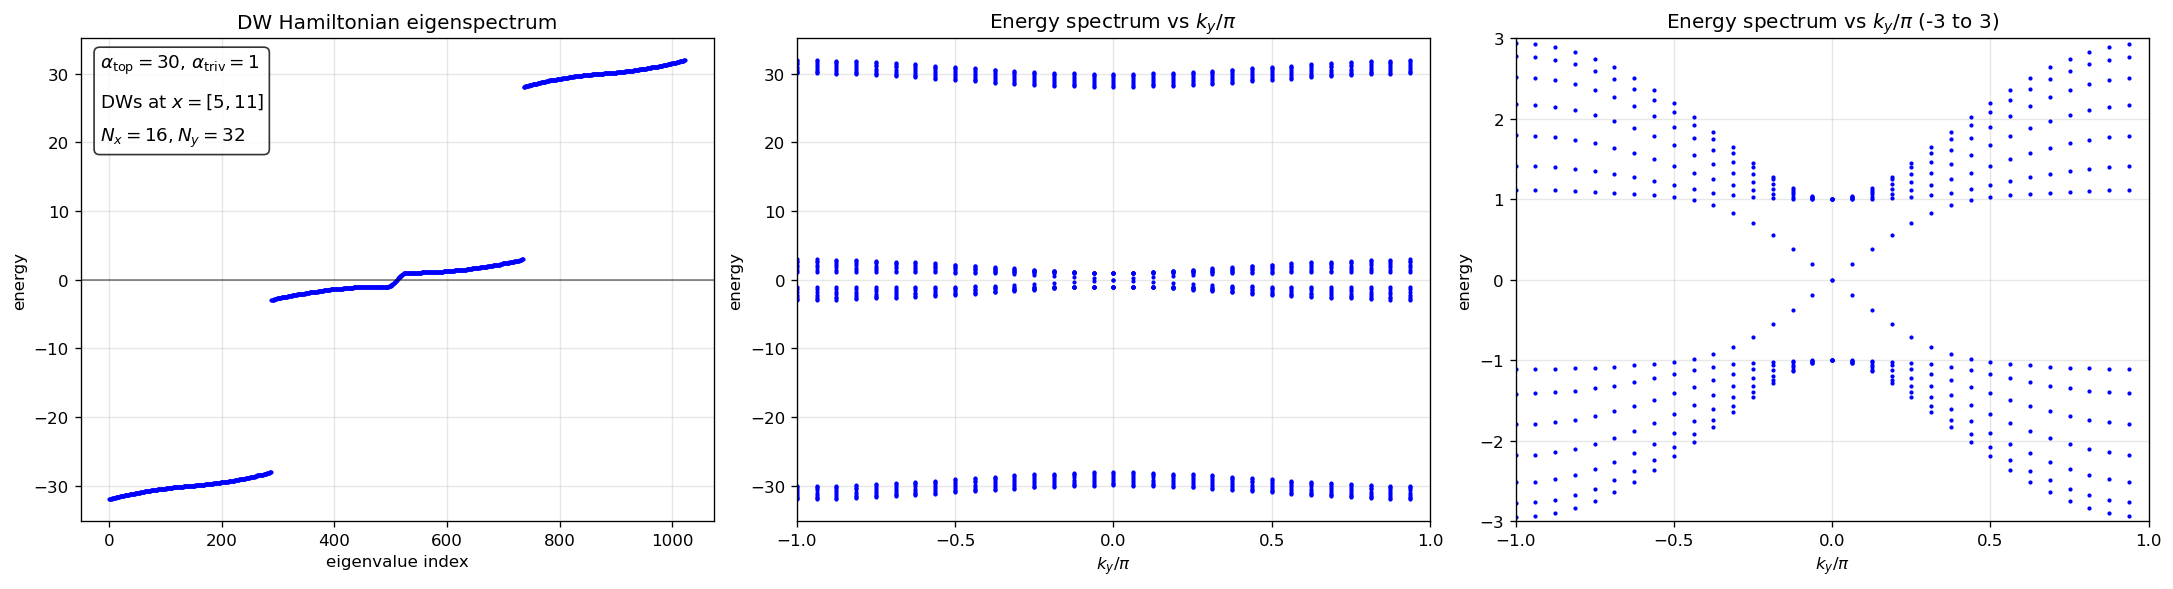
\includegraphics[width=\textwidth]{DW_GS_Benchmark_Figs/output.png}
\caption{
The same three-panel spectral diagnostic as in
Fig.~\ref{fig:energy-main}, but for an alternate benchmark geometry
$N_x=16$, $N_y=32$, with domain walls at $x\in[5,11]$.
This archived figure records an earlier system-size choice used during the
development of the notebook.
}
\label{fig:energy-alt}
\end{figure}

\begin{figure}[t]
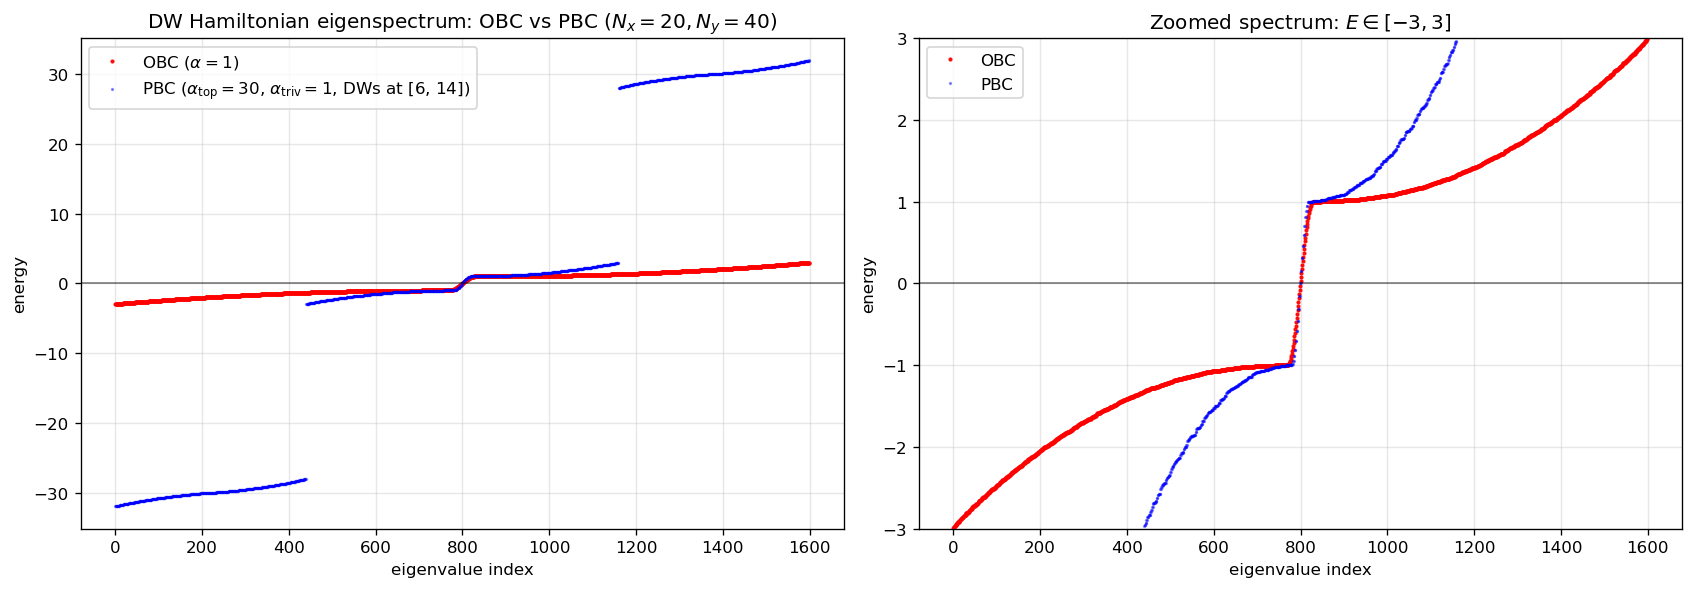
\includegraphics[width=\textwidth]{DW_GS_Benchmark_Figs/energy_spec_pbcs_vs_obcs.png}
\caption{
Comparison between the periodic domain-wall benchmark spectrum (blue) and an
open-boundary reference spectrum (red) used in the notebook.
The left panel shows the full ordered spectrum; the right panel zooms into the
window $E\in[-3,3]$.
}
\label{fig:pbc-obc}
\end{figure}

\section{Reduced Covariance, Entropy, and Entanglement Contour}
Given a subsystem $A$, the notebook forms the reduced covariance by selecting
the corresponding site-orbital indices,
\begin{equation}
G_A = G[\mathrm{idx}(A),\mathrm{idx}(A)].
\label{eq:reduced-cov}
\end{equation}
The associated one-body correlation matrix is
\begin{equation}
C_A = \frac{1}{2}\bigl(\Id_A + G_A\bigr).
\label{eq:corr-matrix}
\end{equation}
If $\{\lambda_n\}$ denotes the spectrum of $C_A$, the von Neumann entropy is
\begin{equation}
S(A)
=
-\sum_n
\Bigl[
\lambda_n \log \lambda_n
+
(1-\lambda_n)\log(1-\lambda_n)
\Bigr].
\label{eq:entropy}
\end{equation}

The notebook's entanglement contour is the diagonal of the operator
\begin{equation}
F_A
=
-C_A\log C_A
-
(\Id_A-C_A)\log(\Id_A-C_A),
\label{eq:contour-operator}
\end{equation}
namely
\begin{equation}
s_A(i) = (F_A)_{ii}.
\label{eq:site-contour}
\end{equation}
Using the two-orbital structure, the contour displayed on the lattice is
\begin{equation}
s_A(x,y)
=
\sum_{\mu=0}^{1}
s_A\bigl(\mu,x,y\bigr),
\label{eq:lattice-contour}
\end{equation}
which obeys the sum rule
\begin{equation}
\sum_{(x,y)\in A} s_A(x,y) = S(A).
\label{eq:sum-rule}
\end{equation}

For the half-system benchmark one chooses
\begin{equation}
A_{1/2}
=
\bigl\{(x,y)\,\big|\,0\le x < N_x,\; y\in Y_{1/2}\bigr\},
\end{equation}
with $Y_{1/2}$ a contiguous block of length $N_y/2$ generated by the helper
\texttt{contiguous\_y\_block}.  The notebook then plots both the full map
$s_{A_{1/2}}(x,y)$ and semilogarithmic cuts at fixed $x$.

\begin{figure}[t]
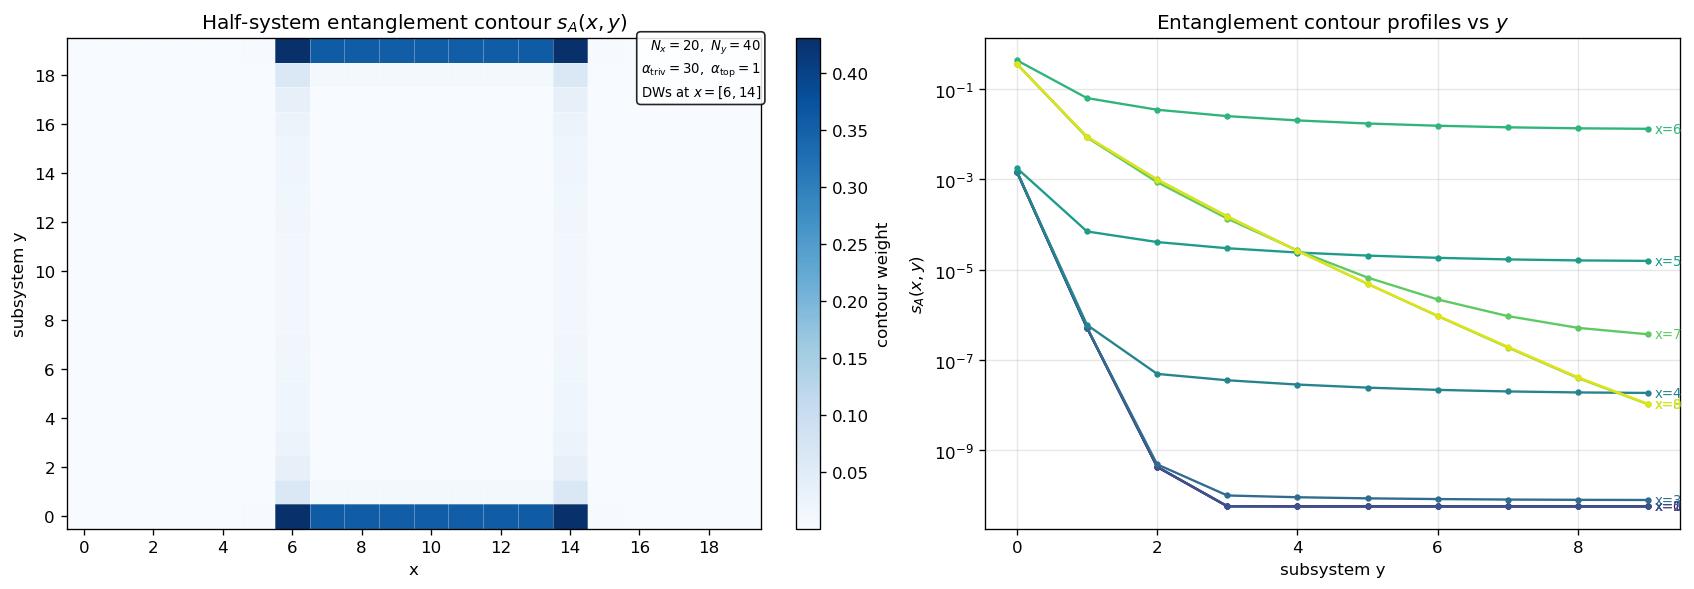
\includegraphics[width=\textwidth]{DW_GS_Benchmark_Figs/ec_heatmap_profiles.png}
\caption{
Entanglement-contour diagnostics for the half-system strip.
Left: the contour map $s_A(x,y)$ on a full-width subsystem of height $N_y/2$.
Right: semilogarithmic profiles $s_A(x,y)$ versus the subsystem coordinate $y$
for several fixed values of $x$.
}
\label{fig:ec-half}
\end{figure}

\section{Fixed-\texorpdfstring{$x$}{x} Squared-Correlation Profiles}
The notebook also studies a boundary-sensitive equal-time two-point diagnostic
constructed from the exact covariance $G_{\mathrm{eq}}$ at fixed $x$.  For a
given slice $x_0$ and $y$ separation $r_y$, it forms the $y$-averaged squared
correlator
\begin{equation}
C_G(x_0,r_y)
=
\frac{1}{N_y}
\sum_{y=0}^{N_y-1}
\sum_{\mu,\nu=0}^{1}
\bigl|
G_{\mathrm{eq}}(x_0,y,\mu;\,x_0,y+r_y,\nu)
\bigr|^2,
\label{eq:squared-corr}
\end{equation}
with $y+r_y$ understood modulo $N_y$.  The left panel of the updated benchmark
figure presents $\log C_G(x_0,r_y)$ versus $\log r_y$ for a representative set
of fixed-$x$ slices.  This broad survey is not intended as a precision fit; it
is a quick way to see which $x$ positions behave edge-like and which do not.

To test chord-length scaling more sharply, the notebook then isolates the
domain-wall slices and their immediate neighbors and re-expresses the horizontal
axis in terms of the periodic chord variable
\begin{equation}
\log \ell_y(r_y),
\qquad
\ell_y(r_y)
=
\frac{N_y}{\pi}
\sin\!\Bigl(\frac{\pi r_y}{N_y}\Bigr).
\label{eq:ry-chord}
\end{equation}
Fits are performed only on the intermediate window $r_y \in [3,15]$, where the
finite-size endpoint effects are visibly reduced.  The figure shows that the
actual domain-wall slices $x=6$ and $x=14$ are extremely well described by a
straight line in $\log C_G$ versus $\log \ell_y$, with fitted slope
$m \approx -2.025$ and $R^2 \approx 0.9998$.  The exterior neighbors
$x=5,15$ behave similarly, with slope $m \approx -2.069$ and
$R^2 \approx 0.9988$.  By contrast, the interior neighbors $x=7,13$ fall much
more steeply, with fit slope $m \approx -13.134$ and noticeably poorer
linearity.  The practical conclusion is therefore that the clean algebraic
chord-length scaling is localized on the domain wall and its immediate exterior
neighbor, whereas slices shifted inward toward the topological strip are already
dominated by much faster decay.

\begin{figure}[t]
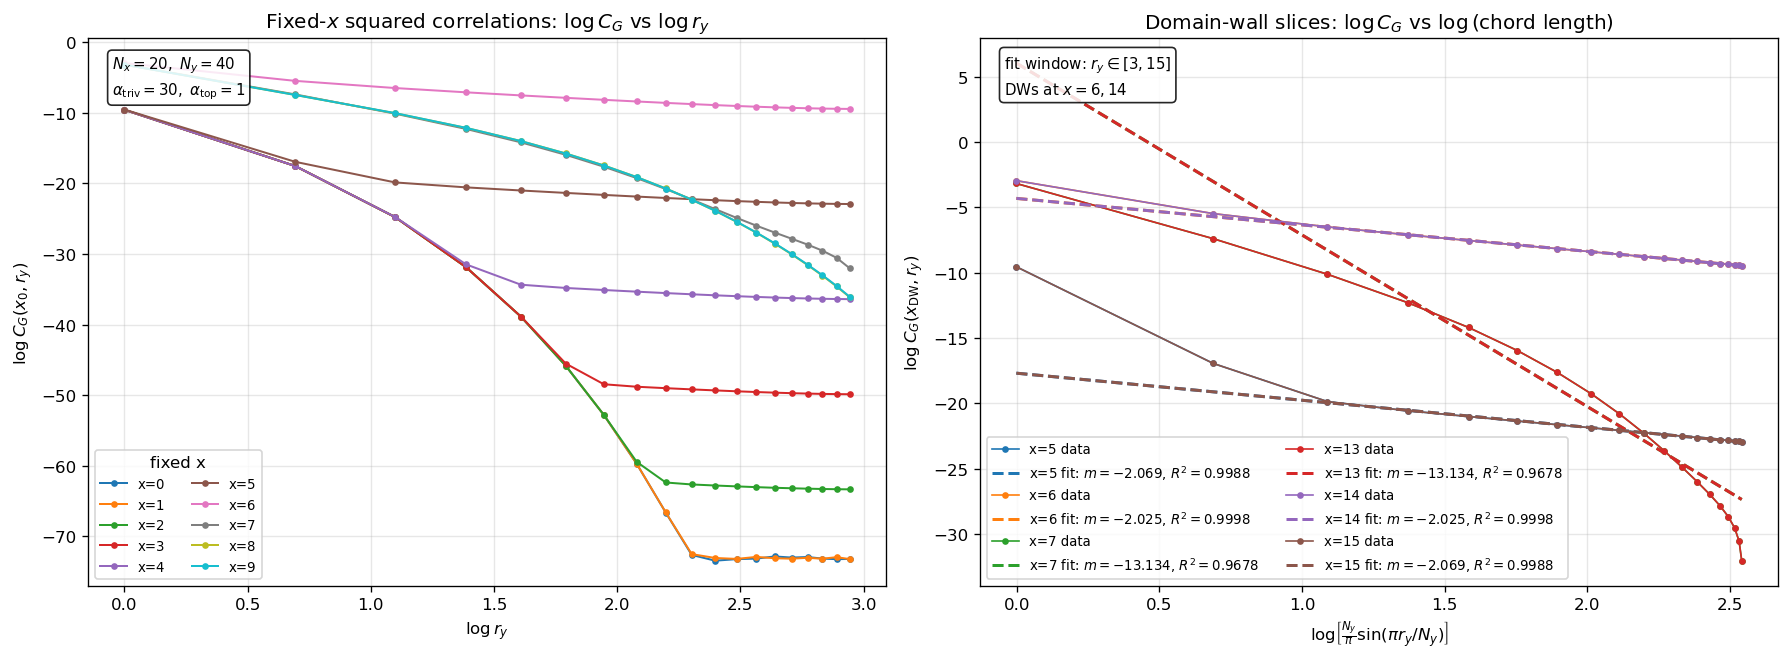
\includegraphics[width=\textwidth]{DW_GS_Benchmark_Figs/square_correlation_profile_y.png}
\caption{
Fixed-$x$ squared-correlation benchmark built from the exact covariance
$G_{\mathrm{eq}}$.
Left: $\log C_G(x_0,r_y)$ versus $\log r_y$ for several fixed-$x$ slices,
showing that the decay profile depends strongly on distance from the domain
walls.
Right: the domain-wall slices and their nearest neighbors plotted against the
logarithm of the periodic chord length \eqref{eq:ry-chord}, together with linear
fits over the window $r_y\in[3,15]$.  The domain-wall slices $x=6,14$ and their
outer neighbors $x=5,15$ are close to a $C_G \sim \ell_y^{-2}$ law, while the
inner neighbors $x=7,13$ decay much more rapidly.
}
\label{fig:square-corr}
\end{figure}

\begin{figure}[t]
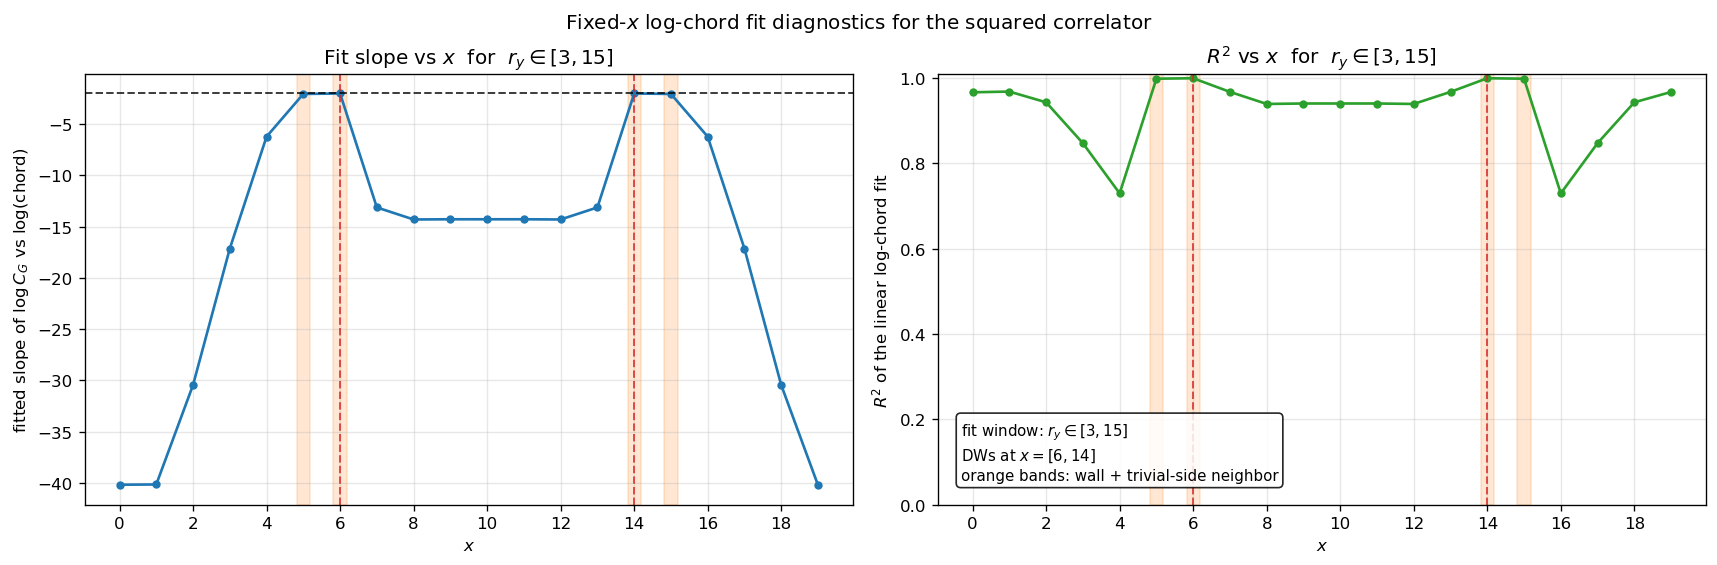
\includegraphics[width=0.9\textwidth]{DW_GS_Benchmark_Figs/square_correlation_profile_y_logchord_fitted_slopes_vs_x.png}
\caption{
Fixed-$x$ log-chord fit diagnostics extracted from the fit window
$r_y\in[3,15]$.
Left: fitted slope of $\log C_G(x,r_y)$ versus $\log \ell_y(r_y)$ as a function
of $x$, with a dashed horizontal reference line at slope $-2$ and vertical
markers at the two domain walls.
Right: the corresponding coefficient of determination $R^2$ as a function of
$x$.
Together these panels show that the near-$-2$ chord-length scaling is sharply
localized on the wall and the trivial-side neighbor: for the left interface the
pair $(x=5,6)$ behaves similarly, while for the right interface the analogous
pair is $(x=14,15)$.
}
\label{fig:square-corr-fit-x}
\end{figure}

To test how much of that edge scaling survives after spatial averaging, the
notebook also forms the uniform $x$ average of the same fixed-slice correlator,
\begin{equation}
C_{\mathrm{avg}}(r_y)
=
\frac{1}{N_x}\sum_{x=0}^{N_x-1} C_G(x,r_y),
\label{eq:squared-corr-xavg}
\end{equation}
and analyzes it on both $\log r_y$ and log-chord axes.  The resulting
$x$-averaged profile is shown in Fig.~\ref{fig:square-corr-xavg}.  Even after
including all $x$ slices, the intermediate-range fit over $r_y\in[3,15]$
remains very close to a straight line in $\log C_{\mathrm{avg}}$ versus
$\log \ell_y$, with slope $m\approx -2.069$ and $R^2\approx 0.9990$.  This is
interesting because the strictly local fit diagnostics of
Fig.~\ref{fig:square-corr-fit-x} show that only a narrow set of slices near the
two interfaces display clean edge-like scaling.  The global average therefore
suggests that those interface-dominated contributions still control the
intermediate-distance behavior of the spatially averaged squared correlator,
even though most individual off-wall slices decay much faster.

\begin{figure}[t]
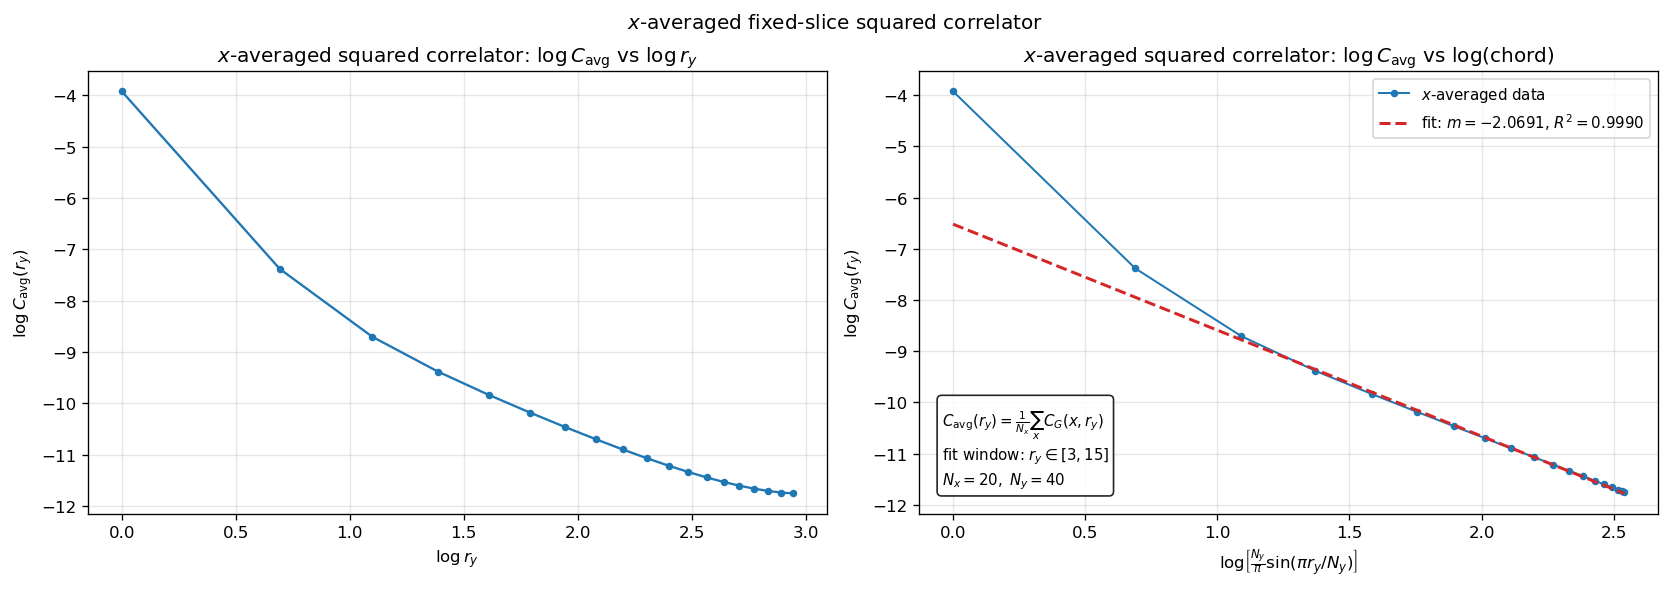
\includegraphics[width=\textwidth]{DW_GS_Benchmark_Figs/x0_avged_square_correlation_profile_y_logchord_fit.png}
\caption{
Uniformly $x$-averaged squared-correlation diagnostic built from the fixed-slice
correlator of Eq.~\eqref{eq:squared-corr}.  Left:
$\log C_{\mathrm{avg}}(r_y)$ versus $\log r_y$, where
$C_{\mathrm{avg}}(r_y)=N_x^{-1}\sum_x C_G(x,r_y)$.  Right: the same averaged
data plotted against the logarithm of the periodic chord length
\eqref{eq:ry-chord}, together with the linear fit over the window
$r_y\in[3,15]$.  The fitted slope remains close to $-2$, indicating that the
domain-wall contribution continues to dominate this averaged observable over the
intermediate distances resolved in the benchmark.
}
\label{fig:square-corr-xavg}
\end{figure}

\section{Lattice and Modular Current Densities}
The current-density constructions used alongside the notebook can be organized
starting from a general quadratic lattice Hamiltonian
\begin{equation}
H
=
\sum_{\bm{r},\bm{r}'}
\Psi_{\bm{r}}^\dagger\, h_{\bm{r}\bm{r}'}\, \Psi_{\bm{r}'},
\qquad
\bm{r}=(x,y),
\label{eq:quadratic-h-general}
\end{equation}
where each block $h_{\bm{r}\bm{r}'}$ is a $2\times 2$ matrix in the orbital
indices $\mu,\nu\in\{0,1\}$.  The cell occupation operator is
\begin{equation}
n_{\bm{r}} = \Psi_{\bm{r}}^\dagger \Psi_{\bm{r}}.
\end{equation}
Using the Heisenberg equation, one finds a lattice continuity equation of the
form
\begin{equation}
\dot{n}_{\bm{r}} + \sum_{\bm{r}'} J_{\bm{r}\to \bm{r}'} = 0,
\label{eq:lattice-continuity}
\end{equation}
with bond-current operator
\begin{equation}
J_{\bm{r}\to \bm{r}'}
=
-\ii\, \Psi_{\bm{r}}^\dagger h_{\bm{r}\bm{r}'} \Psi_{\bm{r}'}
+\ii\, \Psi_{\bm{r}'}^\dagger h_{\bm{r}'\bm{r}} \Psi_{\bm{r}}.
\label{eq:bond-current-operator}
\end{equation}
For a Gaussian state with one-body correlation matrix
\begin{equation}
C_{\bm{r}\bm{r}'}^{\mu\nu}
=
\langle c_{\bm{r},\mu}^\dagger c_{\bm{r}',\nu}\rangle,
\end{equation}
Hermiticity $h_{\bm{r}'\bm{r}}=h_{\bm{r}\bm{r}'}^\dagger$ reduces the
expectation value of Eq.~\eqref{eq:bond-current-operator} to
\begin{equation}
j_{\bm{r}\to \bm{r}'}
=
2\,\mathrm{Im}\,
\mathrm{Tr}\!\Bigl[
h_{\bm{r}\bm{r}'}\, C_{\bm{r}'\bm{r}}
\Bigr].
\label{eq:generic-bond-current}
\end{equation}
Written explicitly in the two-orbital basis,
\begin{equation}
j_{\bm{r}\to \bm{r}'}
=
2\,\mathrm{Im}
\sum_{\mu,\nu=0}^{1}
h_{\bm{r}\bm{r}'}^{\mu\nu}\,
C_{\bm{r}'\bm{r}}^{\nu\mu}.
\label{eq:generic-bond-current-two-orbital}
\end{equation}

On the square lattice of Eqs.~\eqref{eq:realspace-h} and
\eqref{eq:hopping-blocks}, the positively oriented nearest-neighbor currents are
therefore
\begin{align}
j_x(x,y)
&=
2\,\mathrm{Im}\,
\mathrm{Tr}\!\Bigl[
h_{(x,y),(x+1,y)}\,
C_{(x+1,y),(x,y)}
\Bigr],
\label{eq:jx-general}
\\
j_y(x,y)
&=
2\,\mathrm{Im}\,
\mathrm{Tr}\!\Bigl[
h_{(x,y),(x,y+1)}\,
C_{(x,y+1),(x,y)}
\Bigr].
\label{eq:jy-general}
\end{align}
For the physical domain-wall Hamiltonian one simply substitutes the fixed
nearest-neighbor blocks $h_{(x,y),(x+1,y)}=t_x$ and
$h_{(x,y),(x,y+1)}=t_y$ from Eq.~\eqref{eq:hopping-blocks}.  In the code this
is the gauge-fixed lattice-current convention associated with the flattening map
$i(\mu,x,y)=\mu+2x+2N_xy$ and the orbital basis defined in
Eq.~\eqref{eq:bloch-h}.

The same formula applies to modular currents on a subsystem $A$.  From the
reduced covariance Eq.~\eqref{eq:reduced-cov} and correlation matrix
Eq.~\eqref{eq:corr-matrix}, the Gaussian reduced density matrix can be written
as
\begin{equation}
\rho_A \propto \exp\!\bigl[-\Psi_A^\dagger h_A^{\mathrm{mod}}\Psi_A\bigr],
\end{equation}
where the one-body modular Hamiltonian is
\begin{equation}
h_A^{\mathrm{mod}}
=
\log\!\Bigl[(\Id_A-C_A)\, C_A^{-1}\Bigr].
\label{eq:modular-hamiltonian-C}
\end{equation}
Using $C_A=(\Id_A+G_A)/2$, this is equivalently
\begin{equation}
h_A^{\mathrm{mod}}
=
\log\!\Bigl[(\Id_A-G_A)(\Id_A+G_A)^{-1}\Bigr]
=
-2\,\mathrm{arctanh}(G_A),
\label{eq:modular-hamiltonian-G}
\end{equation}
which is the form used by the auxiliary modular-current script.
The modular current density is then obtained by replacing
$h_{\bm{r}\bm{r}'}$ in Eqs.~\eqref{eq:jx-general}--\eqref{eq:jy-general} by the
corresponding blocks of $h_A^{\mathrm{mod}}$, while keeping the same reduced
correlator $C_A$.  Thus the physical and modular current constructions differ
only in the one-body generator inserted into the same continuity-equation
formula.

\section{Local Chern Marker}
Topological structure is probed through the local Chern marker built from the
projector
\begin{equation}
P = \frac{1}{2}\bigl(\Id + G\bigr).
\label{eq:projector-from-G}
\end{equation}
Writing $X$ and $Y$ for the position operators, the notebook evaluates the
six-index operator
\begin{equation}
M = 2\pi \ii \bigl(PXPYP - PYPXP\bigr),
\label{eq:lcm-operator}
\end{equation}
and then defines the site-resolved marker
\begin{equation}
C(x,y)
=
\sum_{\mu=0}^{1}
M_{(x,y,\mu),(x,y,\mu)}.
\label{eq:lcm}
\end{equation}
The stored plot uses the bounded visualization
\begin{equation}
C_{\tanh}(x,y) = \tanh\!\bigl(C(x,y)\bigr).
\label{eq:lcm-tanh}
\end{equation}

\begin{figure}[t]
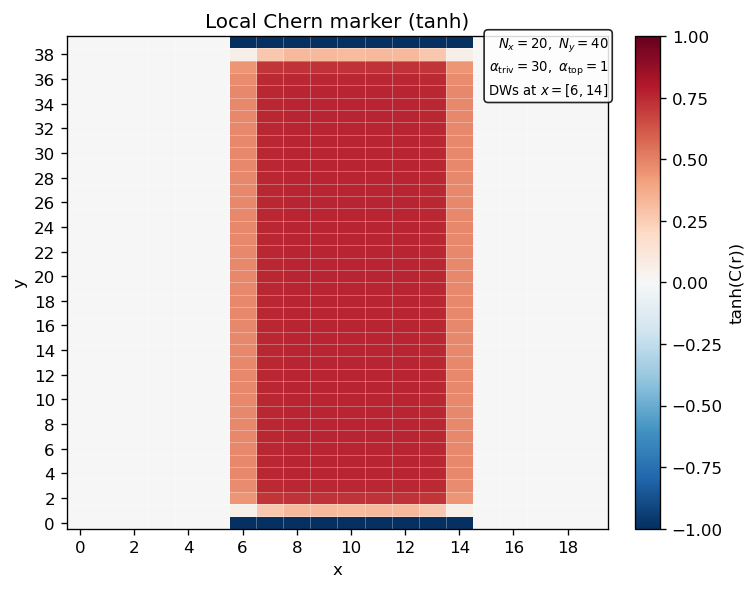
\includegraphics[width=0.62\textwidth]{DW_GS_Benchmark_Figs/chern_marker.png}
\caption{
Tanh-compressed local Chern marker $C_{\tanh}(x,y)$ for the exact Gaussian
ground state.  The nearly quantized domain-wall slab is visibly localized
between the two marked interfaces.
}
\label{fig:chern}
\end{figure}

\section{Integrated Entanglement Contour and Chord-Length Fits}
For the contour benchmark as a function of subsystem height, the notebook fixes
the full-width strip
\begin{equation}
A(\Ay)
=
\bigl\{(x,y)\,\big|\,0\le x < N_x,\; 0\le y < \Ay\bigr\},
\qquad
1 \le \Ay \le N_y-1,
\label{eq:Ay-strip}
\end{equation}
computes the corresponding contour $s_{A(\Ay)}(x,y)$, and only \emph{afterward}
restricts the final sum to a chosen $x$ window $\Ix$.  The integrated quantity
is therefore
\begin{equation}
\mathcal{S}_{\Ix}(\Ay)
=
\sum_{x\in \Ix}\;
\sum_{y=0}^{\Ay-1}
s_{A(\Ay)}(x,y).
\label{eq:integrated-contour}
\end{equation}
This distinction is crucial: the subsystem itself remains full width in $x$,
while the interval $\Ix$ serves only as a diagnostic window for where the
entanglement contour is spatially concentrated.

To test the expected one-dimensional edge scaling, the notebook separates
Eq.~\eqref{eq:integrated-contour} into the two branches
\begin{equation}
\Ay < \frac{N_y}{2},
\qquad
\Ay > \frac{N_y}{2},
\end{equation}
because the map
\begin{equation}
\Ay \longmapsto \log\!\Bigl[\sin\!\Bigl(\frac{\pi \Ay}{N_y}\Bigr)\Bigr]
\label{eq:log-chord-var}
\end{equation}
is not one-to-one on the full interval $1\le \Ay \le N_y-1$.
Each branch is then fit to
\begin{equation}
\mathcal{S}_{\Ix}(\Ay)
\simeq
m_{\Ix}\,
\log\!\Bigl[\sin\!\Bigl(\frac{\pi \Ay}{N_y}\Bigr)\Bigr]
+
b_{\Ix}.
\label{eq:contour-fit}
\end{equation}

\begin{figure}[t]
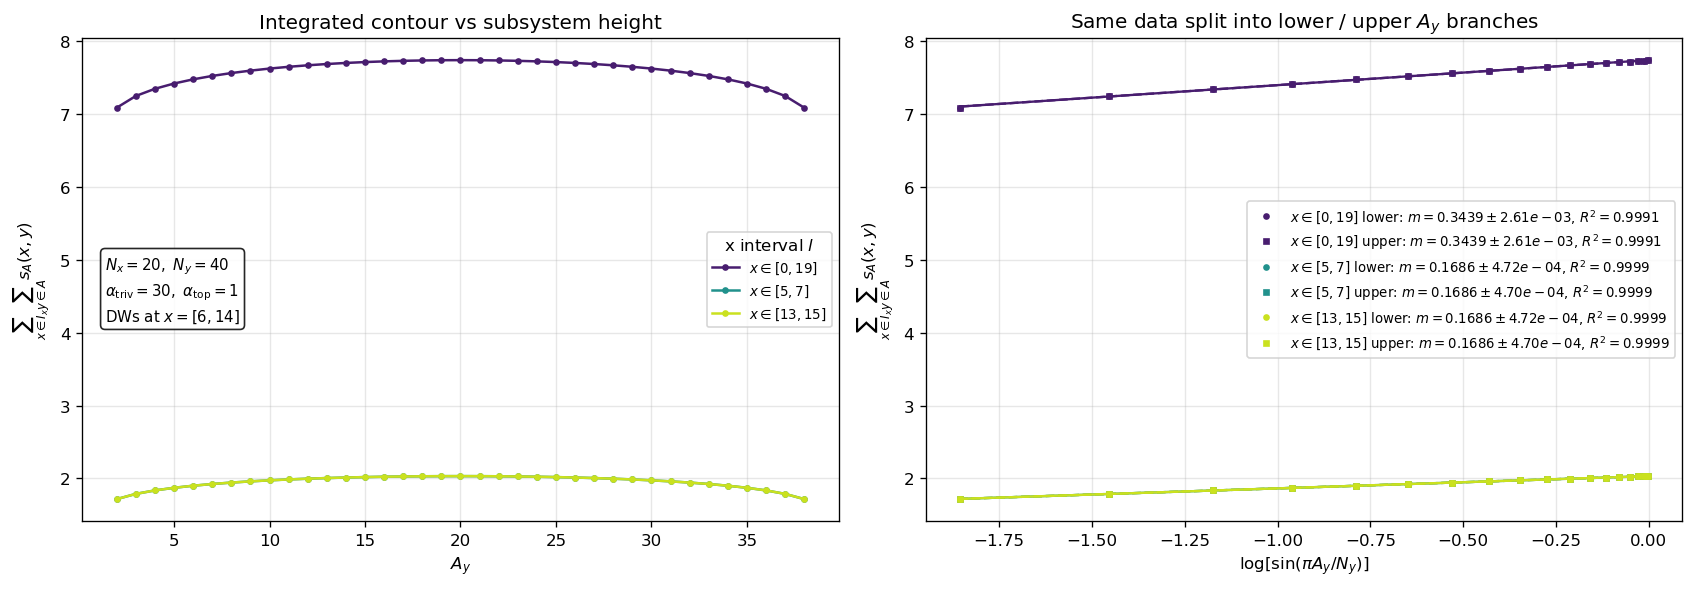
\includegraphics[width=\textwidth]{DW_GS_Benchmark_Figs/integrated_contour_vs_log_chord.png}
\caption{
Integrated contour benchmark.
Left: $\mathcal{S}_{\Ix}(\Ay)$ for the full-width sum and for two narrow
domain-wall-centered windows.
Right: the same data split into lower and upper $\Ay$ branches and fit to the
log-chord form \eqref{eq:contour-fit}.
}
\label{fig:int-contour}
\end{figure}

\section{Flattened-Hamiltonian Trial-Orbital Benchmark}
The notebook also benchmarks an overcomplete-Wannier surrogate for the exact
ground-state covariance by first constructing a flattened single-particle
Hamiltonian from the trial-orbital projectors generated by
\texttt{construct\_OW\_projectors}.  For a choice of trial spinor
$\tau \in \{\sigma_X,\sigma_Y,\sigma_Z\}$, the notebook forms
\begin{equation}
H_{\flat}^{(\tau)}
=
\sum_{R}
\Bigl[
P_{A,R}^{+(\tau)} + P_{B,R}^{+(\tau)}
-
P_{A,R}^{-(\tau)} - P_{B,R}^{-(\tau)}
\Bigr],
\label{eq:hflat}
\end{equation}
followed by an explicit Hermitization,
\begin{equation}
H_{\flat}^{(\tau)} \longrightarrow
\frac{1}{2}\Bigl(H_{\flat}^{(\tau)} + H_{\flat}^{(\tau)\dagger}\Bigr).
\label{eq:hflat-herm}
\end{equation}
After diagonalizing
\begin{equation}
H_{\flat}^{(\tau)} v_n^{(\tau)} = \varepsilon_n^{(\tau)} v_n^{(\tau)},
\end{equation}
it defines the occupied projector
\begin{equation}
P_{\mathrm{occ}}^{(\tau)}
=
\sum_{\varepsilon_n^{(\tau)}<0}
\left|v_n^{(\tau)}\right\rangle \left\langle v_n^{(\tau)}\right|,
\label{eq:pocc-flat}
\end{equation}
and then uses the same flattened covariance convention as in the exact
benchmark,
\begin{equation}
G_{\flat}^{(\tau)} = 2P_{\mathrm{occ}}^{(\tau)} - \Id.
\label{eq:gflat}
\end{equation}
These trial-orbital covariances are then passed through exactly the same
entanglement-contour pipeline as the exact $G_{\mathrm{eq}}$.

The motivation for this surrogate is dynamical as well as variational.  If the
post-selected circuit and the adaptive circuit relax to the same steady state,
then the relaxation time of the adaptive dynamics is bounded from below by the
post-selected relaxation rate.  In that case, understanding the slow approach
to the steady state can be reduced, at least at the level of a lower bound, to
understanding the effective post-selected generator encoded by the flattened
Hamiltonian.  The notebook therefore uses $H_{\flat}^{(\tau)}$ as a controlled
proxy for the long-time structure that may govern slow purification.

A second motivation is that, because the construction is based on
overcomplete-Wannier orbitals rather than exact band projectors, the resulting
spectrum is not perfectly flat.  Instead it is modulated by the
$L^2$-normalized form factor of the chosen Wannier envelope.  This makes the
trial-orbital dependence physically informative rather than merely cosmetic:
different choices of $\tau$ probe how sensitive the surrogate edge theory is to
the spatial and orbital structure built into the OW ansatz.

Figure~\ref{fig:flat-spec} summarizes the single-particle spectra of
$H_{\flat}^{(\tau)}$.  The $\tau\in\sigma_X$ and $\tau\in\sigma_Y$ choices are
nearly indistinguishable: both show a strongly flattened ordered spectrum with
most eigenvalues clustered near $\pm 2$, together with a pair of dispersing
$k_y$-resolved branches crossing near zero.  By contrast,
$\tau\in\sigma_Z$ produces a much broader spectrum, extending to roughly
$\pm 4$, and a visibly different $k_y$-resolved band structure.  In that sense
the $X$ and $Y$ trial spinors generate very similar OW surrogates, whereas the
$Z$ choice is spectrally distinct already at the level of the flattened
Hamiltonian.

\begin{figure}[t]
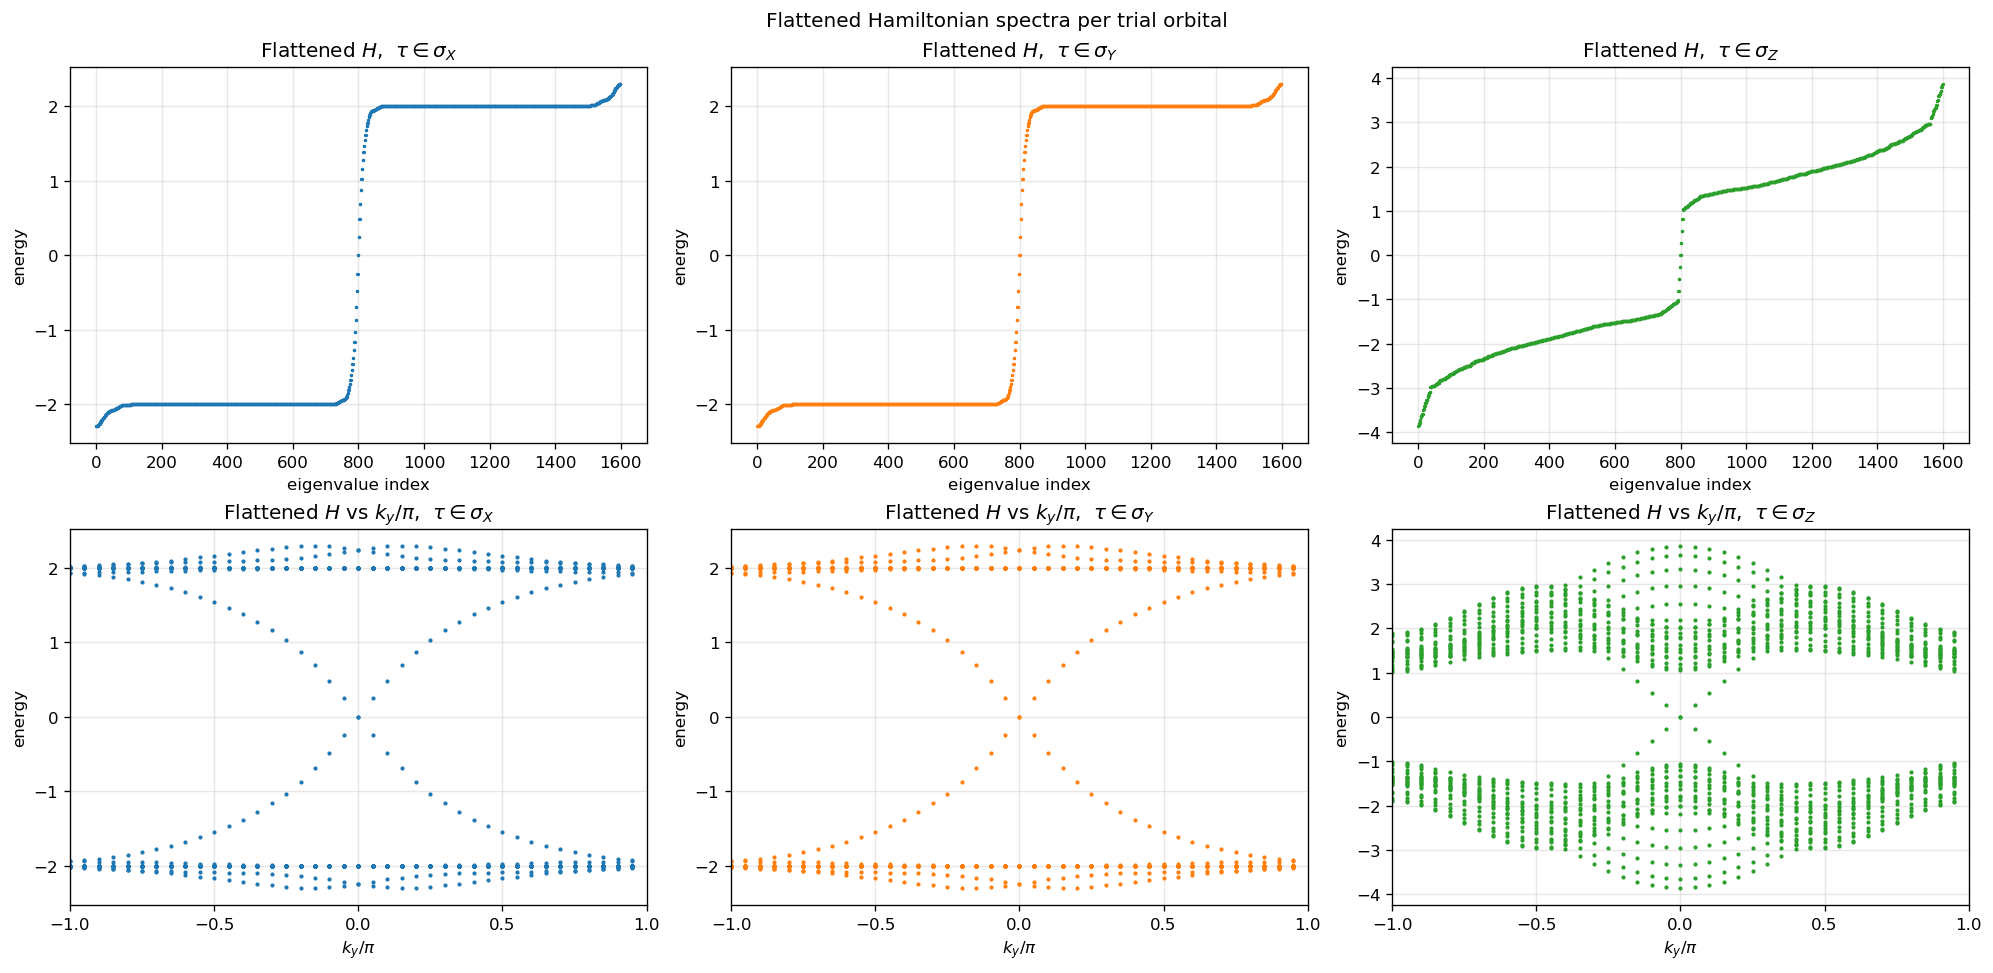
\includegraphics[width=\textwidth]{DW_GS_Benchmark_Figs/flattened_hamiltonian_spec.png}
\caption{
Spectra of the OW flattened Hamiltonian $H_{\flat}^{(\tau)}$ for the three
trial-orbital choices $\tau\in\sigma_X,\sigma_Y,\sigma_Z$.
Top row: ordered eigenvalues of the Hermitized matrix \eqref{eq:hflat-herm}.
Bottom row: spectra of the corresponding $k_y$-resolved blocks, obtained by the
same Fourier-block decomposition used for the exact benchmark.
The $X$ and $Y$ trial orbitals lead to nearly identical flattened spectra,
whereas the $Z$ choice is appreciably broader and more dispersive.
}
\label{fig:flat-spec}
\end{figure}

The entanglement benchmark based on these trial-orbital covariances is shown in
Figs.~\ref{fig:flat-ent} and \ref{fig:flat-ent-fit}.  For each
$G_{\flat}^{(\tau)}$, the notebook computes the full-width contour on the strip
$A(\Ay)=[0,N_x)\times[0,\Ay)$ and then integrates the resulting contour over
the same three $x$ windows used in the exact benchmark:
the full width $\Ix=[0,N_x-1]$ and the two three-site windows centered on the
domain walls.  The raw $\Ay$-dependence in Fig.~\ref{fig:flat-ent} already
shows that all three trial-orbital constructions track the exact benchmark
closely.

\begin{figure*}[t]
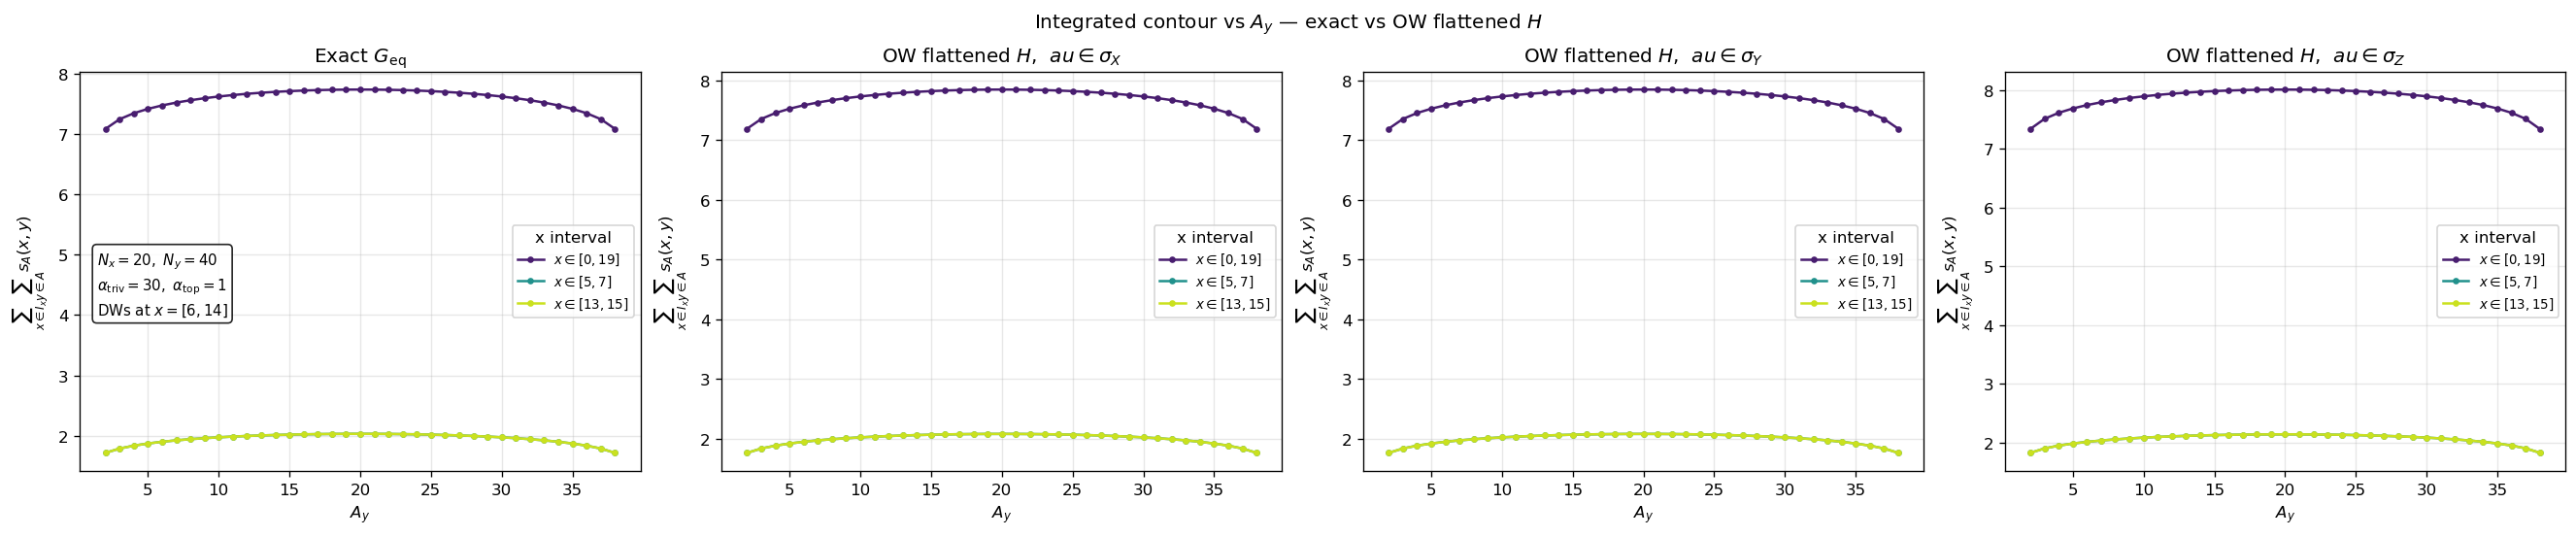
\includegraphics[width=\textwidth]{DW_GS_Benchmark_Figs/flattened_hamiltonian_entanglement.png}
\caption{
Integrated contour curves
$\mathcal{S}_{\Ix}(\Ay)=\sum_{x\in\Ix}\sum_{y=0}^{\Ay-1}s_{A(\Ay)}(x,y)$
for the exact covariance and for the three trial-orbital flattened-H
covariances.  The four panels compare the full-width diagnostic window and the
two domain-wall-centered windows used in the exact benchmark.
Across all three choices of $\tau$, the raw contour profiles remain close to
the exact curves.
}
\label{fig:flat-ent}
\end{figure*}

The more discriminating comparison comes from the branch-by-branch log-chord
fits.  Figure~\ref{fig:flat-ent-fit} shows that the $X$ and $Y$ trial orbitals
reproduce the exact fitted slopes extremely well.  For the full-width interval,
the exact benchmark gives $m\approx 0.3439$, while the $X$ and $Y$ trial
orbitals give $m\approx 0.3448$.  For the two domain-wall-centered windows, the
exact slope is $m\approx 0.1686$ on both branches, compared with
$m\approx 0.1691$ for $X$ and $Y$.  The $\tau\in\sigma_Z$ construction still
shows the same qualitative additivity of two nearly equal wall contributions,
but its slopes are more noticeably shifted, to about $0.3511$ on the full-width
window and $0.166$--$0.167$ on the narrow wall windows.  Thus the integrated
entanglement-contour scaling is quite robust under the OW approximation, with
$X$ and $Y$ performing especially well and $Z$ remaining qualitatively correct
but quantitatively less accurate.

\begin{figure*}[t]
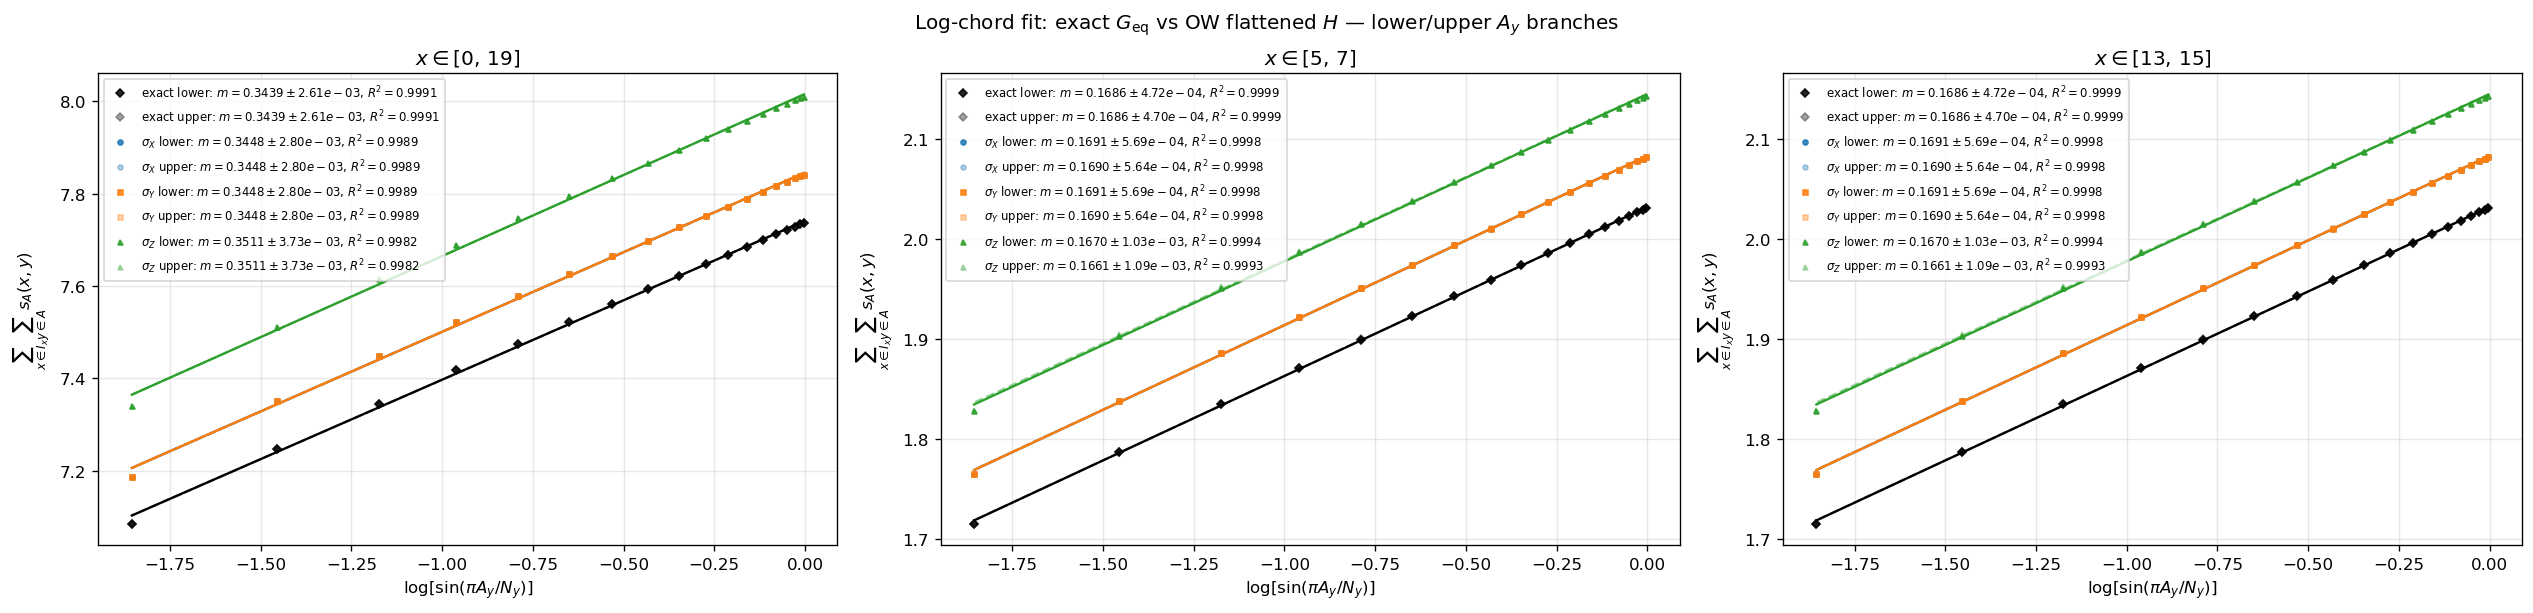
\includegraphics[width=\textwidth]{DW_GS_Benchmark_Figs/flattened_hamiltonian_entanglment_log_chord_fits.png}
\caption{
Lower- and upper-branch log-chord fits of the integrated contour for the exact
covariance and the three OW flattened-H trial-orbital constructions.
Each panel corresponds to one $x$ interval: full width, left domain wall, and
right domain wall.  The $X$ and $Y$ trial orbitals reproduce the exact fit
slopes almost indistinguishably, while the $Z$ trial orbital shows a larger but
still controlled deviation.
}
\label{fig:flat-ent-fit}
\end{figure*}

\section{Contour-Restricted Mutual-Information Diagnostics}
The notebook also implements a multipartite diagnostic adapted from
\texttt{analysis.ipynb}.  One chooses three contiguous intervals in the
$y$ direction,
\begin{equation}
A,\qquad B,\qquad C,
\end{equation}
of lengths $\LA$, $\LB$, and $\LC$, respectively, and either fixes their anchor
$y_0$ or averages over all $y_0$ translations around the $y$ circle.  The
subsystems remain full width in $x$; the chosen interval $\Ix$ is applied only
in the final contour sum.

For any $y$ region $Y$, let $s_Y(x,y)$ denote the contour computed on the
full-width subsystem associated with $Y$.  The notebook then defines the
contour-restricted entropy proxy
\begin{equation}
S^{(\Ix)}(Y)
=
\sum_{x\in \Ix}\;
\sum_{y\in Y}
s_Y(x,y).
\label{eq:partialx-entropy}
\end{equation}
From these quantities it constructs
\begin{align}
I_2^{(\Ix)}(A:C)
&=
S^{(\Ix)}(A) + S^{(\Ix)}(C) - S^{(\Ix)}(AC),
\label{eq:I2}
\\
I_3^{(\Ix)}(A:B:C)
&=
S^{(\Ix)}(A)+S^{(\Ix)}(B)+S^{(\Ix)}(C)
\nonumber\\
&\quad
-S^{(\Ix)}(AB)-S^{(\Ix)}(AC)-S^{(\Ix)}(BC)
+S^{(\Ix)}(ABC).
\label{eq:I3}
\end{align}
The benchmark emphasizes the difference
\begin{equation}
\Delta I^{(\Ix)} \equiv I_2^{(\Ix)} - I_3^{(\Ix)}.
\label{eq:deltaI}
\end{equation}

To compare with a one-dimensional conformal variable, the notebook uses the
chord length
\begin{equation}
\ell(L) = \frac{N_y}{\pi}\sin\!\Bigl(\frac{\pi L}{N_y}\Bigr),
\label{eq:chord}
\end{equation}
and the cross ratio
\begin{equation}
x
=
\frac{\ell(\LA)\,\ell(\LC)}
{\ell(\LA+\LB)\,\ell(\LB+\LC)}.
\label{eq:cross-ratio}
\end{equation}
The final linear fit is performed against
\begin{equation}
\Delta I^{(\Ix)}(x)
\simeq
m_{\Ix}\,\log\!\Bigl(\frac{1}{1-x}\Bigr)
+
b_{\Ix}.
\label{eq:MI-fit}
\end{equation}

\begin{figure}[t]
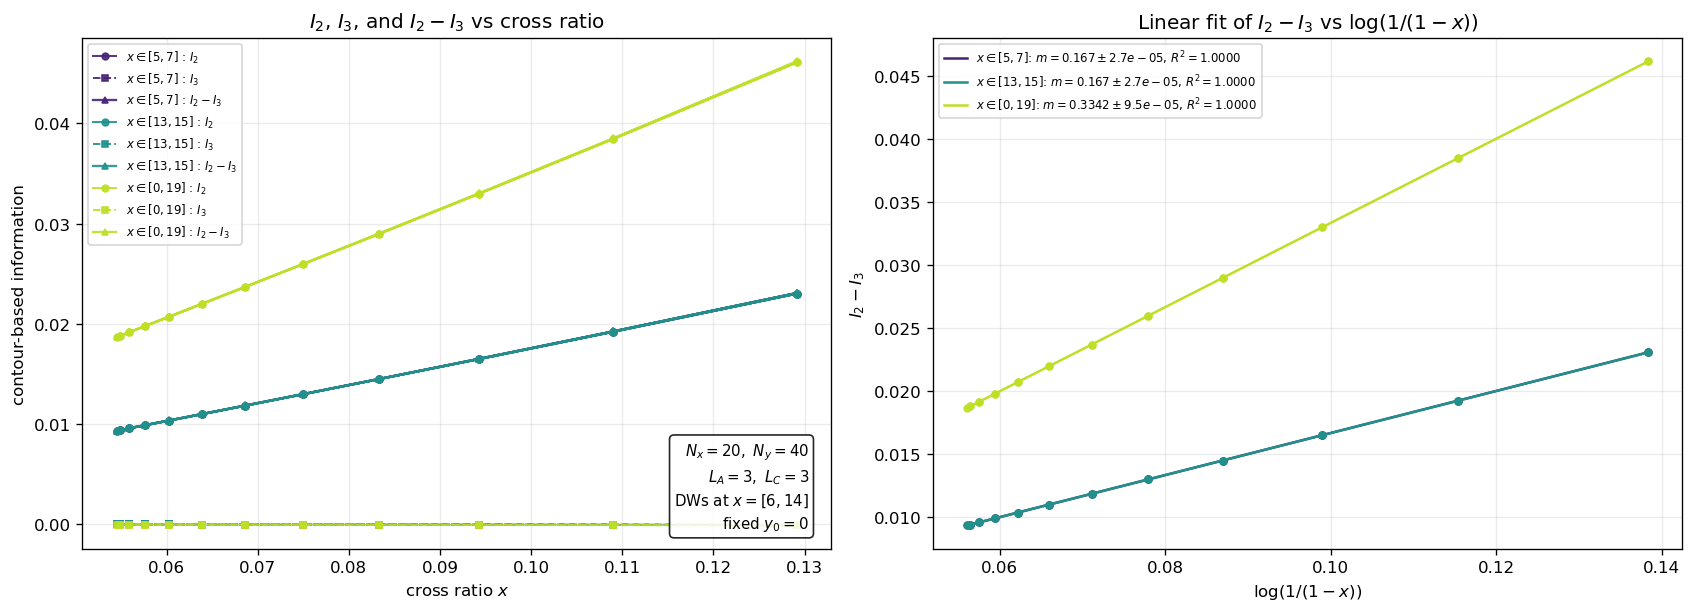
\includegraphics[width=\textwidth]{DW_GS_Benchmark_Figs/MI_linear_fits.png}
\caption{
Contour-restricted multipartite-information benchmark for three different
$x$ windows.
Left: $I_2^{(\Ix)}$, $I_3^{(\Ix)}$, and $\Delta I^{(\Ix)}=I_2^{(\Ix)}-I_3^{(\Ix)}$
plotted against the cross ratio \eqref{eq:cross-ratio}.
Right: linear fits of $\Delta I^{(\Ix)}$ against $\log(1/(1-x))$.
}
\label{fig:MI-fit}
\end{figure}

\begin{figure}[t]
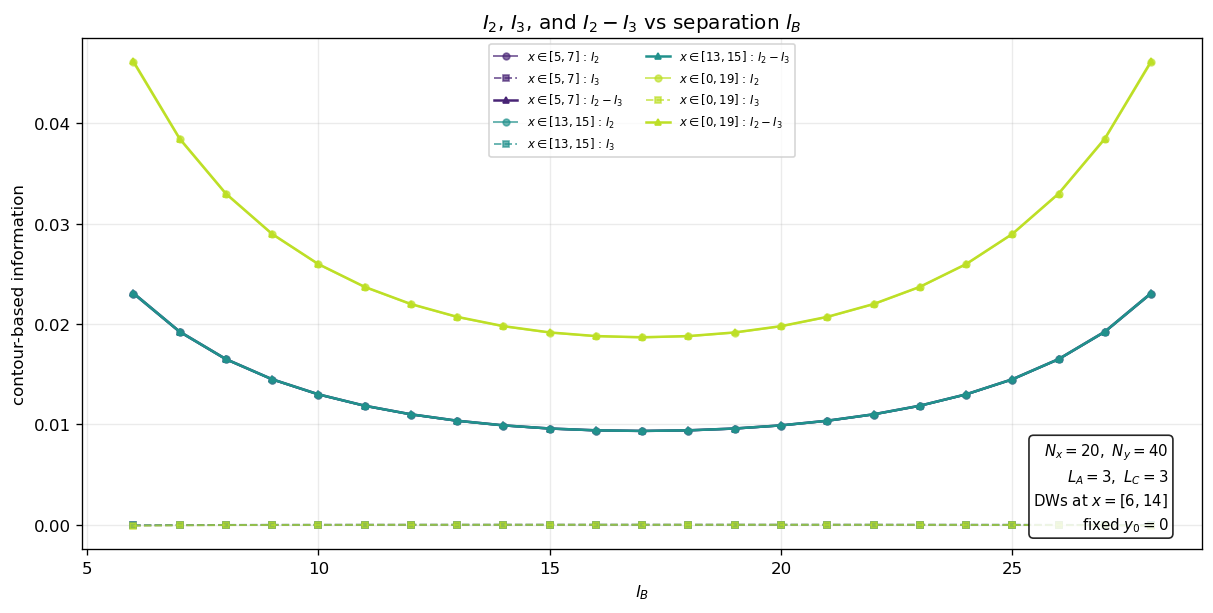
\includegraphics[width=\textwidth]{DW_GS_Benchmark_Figs/MI_vs_B.png}
\caption{
The same contour-restricted information measures displayed directly as functions
of the separation $\LB$ between the two outer intervals of lengths $\LA$ and
$\LC$.  The figure illustrates how the signal depends on the choice of the
post-contour $x$ window.
}
\label{fig:MI-B}
\end{figure}

\section{Ancillary Benchmark Metrics}
Although the presently saved figure set does not include the dynamic-state
comparison cell, the notebook helper layer also defines two standard diagnostics
for comparing a dynamically prepared covariance $G_{\mathrm{dyn}}$ against the
equilibrium benchmark $G_{\mathrm{eq}}$.

First, the Frobenius mismatch is
\begin{equation}
\|G_{\mathrm{eq}} - G_{\mathrm{dyn}}\|_F
=
\sqrt{
\operatorname{Tr}
\Bigl[
\bigl(G_{\mathrm{eq}} - G_{\mathrm{dyn}}\bigr)^{\dagger}
\bigl(G_{\mathrm{eq}} - G_{\mathrm{dyn}}\bigr)
\Bigr]
}.
\label{eq:frob}
\end{equation}
Second, the notebook defines a site-resolved difference map by reshaping the
matrix difference into a six-index tensor and tracing its squared modulus over
all source and orbital indices,
\begin{equation}
d(x,y)
=
\Biggl[
\sum_{\mu,\nu,x',y'}
\left|
\Delta G_{\mu,x,y;\nu,x',y'}
\right|^2
\Biggr]^{1/2},
\qquad
\Delta G = G_{\mathrm{eq}} - G_{\mathrm{dyn}}.
\label{eq:site-diff}
\end{equation}
These metrics are natural Gaussian benchmarks should the dynamic-preparation
portion of the notebook be reactivated.

\section{Closing Remarks}
The benchmark notebook is conceptually simple but diagnostically rich.
Everything begins from the exact Gaussian ground state of the real-space
Hamiltonian \eqref{eq:realspace-h}, yet the subsequent observables resolve the
same state in complementary ways: by ordered single-particle energies, by
$k_y$-resolved spectral blocks, by fixed-$x$ squared-correlation profiles, by
the local entropy density encoded in the entanglement contour, by the local
Chern response, by strip-integrated log-chord scaling, and by
contour-restricted multipartite information.

For practical use, the most important structural point is the following.
Whenever the notebook loops over an $x$ interval, the intended construction is
usually \emph{not} to redefine the subsystem in $x$; rather, one computes the
entanglement contour on a subsystem that is full width in $x$ and only then
restricts the final sum to a post-processed window $\Ix$.  This is precisely the
convention encoded in Eqs.~\eqref{eq:integrated-contour} and
\eqref{eq:partialx-entropy}, and it is the convention that gives the cleanest
physical interpretation of the benchmark figures.

\end{document}
